\chapter{Introduction}
\label{c_intro}

\section{Motivation}
\label{s_motivation}

Thermonuclear fusion has the potential to solve the world's energy problems. The fusion of a pair of light nuclei, such as deuterium and tritium, releases more energy than the fission
of a uranium nucleus and much more energy than the chemical reactions involved in the burning of fossil fuels. Furthermore, the fusion products 
-- unlike those from nuclear fission and fossil fuel burning-- are relatively harmless to the environment, and fusion fuel sources are much more abundant than fossil fuels
and fissionable uranium. The limiting component of deuterium-tritium fusion reactions is the tritium, which can be made from lithium. Yet there is enough lithium on Earth to power the world
through nuclear fusion for at least a million years~\cite{wesson2004}.

Due to its great potential, scientists have been working on controlling fusion reactions for over half a century. The community has made much progress, but fusion is not yet a commercially
viable energy source, and there are still several scientific and technological obstacles to overcome before it is. The main obstacle to achieving controlled fusion reactions is the confinement of the
reaction fuel for a long enough time at sufficiently high temperatures and densities to achieve a self-sustaining reaction. 
One of the best ways to contain the fuel is to maintain it in a plasma state and restrict the motion of the plasma using magnetic fields. 
Possibly the best way to do this -- and certainly the most intensely studied -- is by using a tokamak. Tokamaks around the world have already achieved temperatures and pressures
necessary to produce fusion but have yet to confine the plasmas for long enough to achieve a self-sustained fusion reaction. Seemingly, this problem can be solved by making
the tokamaks larger, although it's still unclear if the large tokamaks will be able to operate in a high confinement mode (H-mode), which will probably be necessary in order to
keep the tokamaks economically viable. It's also unclear if the material walls of the larger tokamaks will be able to survive the large plasma fluxes.

The plasma confinement time, for a given sized tokamak, is inversely proportional to the rate of cross-field transport in the tokamak, so it's important to know how to minimize that
transport. Now, while the energy transport must be minimized, fusion product alpha particles (and other non-intrinsic impurities) must be transported out of the core so particle transport
must be kept sufficiently high. The cross-field particle and energy transport is primarily driven by microturbulence, which is driven by instabilities due to the presence of free energy sources.
These free energy sources are due to non-Maxwellian velocity-space features of the distribution functions, spatial inhomogeneity of the distribution functions, and stored electromagnetic energy.
These energy sources always exist in the normal operating conditions of a tokamak. For example temperature gradients must exist in tokamaks
since the hot tokamak core cannot extend all the way to the walls, which are kept close to room temperature. In fact, we must take great care in order to prevent a high flux of extremely
hot plasma from hitting the material walls, which can melt them or sputter atoms into the core. 
Transport can actually help in this regard by spreading out the plasma beam that crosses the last-closed-flux-surface so that its flux
per unit area hitting material limiters and divertor targets is reduced. Altogether, turbulent transport is needed in some ways, but is detrimental in other ways. A balance may be key,
or maybe clever techniques and engineering can be used to control the transport in the necessary ways. In either case, it's important to be able to predict how the turbulence and the
transport will react to changes in design or changes in operational parameters. 

Predicting transport has been a long, slow research activity for some time. One large problem is that turbulence is not completely understood even in neutral fluids,
let alone in tokamak plasmas. Nevertheless, at this point, many aspects of turbulence and transport in the tokamak core are fairly well-understood, largely
due to the success of gyro-kinetic simulations. Turbulence in the edge, on the other hand, is not as well-understood for several reasons. One, the edge region contains complex magnetic
field geometry, where the field lines range from open to closed, the open ones ending on material surfaces. Two, turbulent fluctuations are high, invalidating current forms of the
gyro-kinetic equations, leaving no model to absolutely apply to the entire edge region. Three, the edge contains a zoo of potential instabilities that can drive the turbulence,
and seemingly different instabilities exist in different tokamaks and in different operating regimes.

Numerical simulations have helped improve understanding of physical processes and spatial and temporal structures in all kinds of turbulent settings. However,
experimental observations and analytic theory generally lead tokamak research, with simulations merely trying to confirm the ideas obtained from these more established methods.
Nevertheless, simulations can produce more detailed results than analytic theory and more spatial information than experimental observation, making them valuable.
Furthermore, the hope is that simulations can lead experiment, providing predictions before experiments are done, or at least providing enough physical insight to direct experimental efforts.
In some instances, like in the cores of tokamaks, the community has made enough progress on simulations (specifically gyro-kinetic ITG simulations) that simulations have uncovered new
unexpected physics (such as the Dimits shift of ITG turbulence~\cite{dimits2000}). But in other instances, like in the edge of tokamaks, nonlinear turbulent simulations don't yet
agree enough with experiment to provide good physical insight, let alone predictive capabilities. A possible path to making progress on this problem is to reduce the problem
to a simpler one, achieve simulation validation with that, and then slowly move up to more and more complex situations. A natural place to start is simulation of linear plasma devices.

Magnetic plasma devices that are simpler and colder than tokamaks, like the Large Plasma Device (LAPD) at UCLA~\cite{Gekelman1991}, have long been used to study basic plasma processes that
are relevant to tokamaks. These machines, which generally produce plasma turbulence, offer a more experimentally accessible environment than a tokamak. They are also easier to
understand due to their relative simplicity, especially with regard to their magnetic field configurations, which also reduces the number of instabilities present in them. 
Furthermore, they are colder and thus more collisional than tokamaks, making fluid equations more applicable than they are in tokamaks. It should be easier to produce a verified, validated
simulation of turbulence in a linear machine like LAPD than in a tokamak. And any insight gained from analysis of the simulation may apply to tokamak edge turbulence as well, or at least
provide methods of analysis or ideas that may be checked when tokamak simulations become more successful.

\section{Dissertation Summary}
\label{s_summary}

This dissertation focuses on direct simulation and analysis of low frequency turbulent fluctuations in LAPD. Thus, in order to introduce important concepts that I will use, 
in Chapter~\ref{c_turb_and_inst}, I briefly describe the modern paradigm of turbulence. I touch on the statistical Kolmogorov theory that has dominated the history of turbulence investigation,
but I emphasize the newer deterministic turbulence theory that allows for the description of turbulence
by a system of deterministic, dynamical, differential equations. The deterministic theory revolves around solution sets of the nonlinear differential equations called attractors, and in particular,
strange attractors, which give turbulence its random-looking properties. These attractors can have different phase space dimension, and when their dimension is high, the turbulence can be too
difficult to describe with the deterministic theory, so that the statistical theory must be used. The statistical theory is based on different scales of fluctuations or eddies and how they
interact with the background and with each other. I focus primarily on the instability interactions that drive the turbulence using the free energy contained in the equilibrium profile gradients.
Since I find that the turbulence in LAPD is driven by a nonlinear instability with a subcritical flavor, I review the concept of subcritical instability.

After this brief introduction to turbulence concepts, I go on to describe the simulations that I use to reproduce the turbulence in LAPD. In Chapter~\ref{c_braginskii}, I review
the plasma fluid model that I use in the LAPD simulations. Since LAPD has low temperature ($T_e \le 10$ eV and $T_i \le 1$ eV) and is very long,
it is highly collisional, making it suitable for modeling with fluid equations. Thus, I use the Braginskii two-fluid model for the equations, but I use only four of the equations,
neglecting ion temperature, sound waves, and magnetic field fluctuations. Then, in Chapter~\ref{c_lapd_sim}, I show the equations as they appear in the simulations, and I
discuss my methods for numerically reproducing realistic LAPD turbulence. Specifically, I separate the independent variables into time-independent (equilibrium) and time-dependent (fluctuating)
components. I then take the equilibrium density, electron temperature, and magnetic field profiles from experimental measurements, linearize the equations, and then insert back
only the advective nonlinearities into the equations. I simulate a particular LAPD experiment in which the equilibrium radial electric field is nearly zero, allowing me to disregard it.
I show simulation results of non-zero radial electric field experiments in Appendix~\ref{app_mean_flow}, but don't cover them in the main text.
Furthermore, in the simulations, I use ad hoc density and electron temperature sources to maintain the equilibrium gradient drive over time, I use artificial diffusion and viscosity for saturation,
and I use a number of different idealized axial boundary conditions.
As for performing the simulations, I use the BOUT++ code, for which I provide details in Appendix~\ref{app_bout}.

\begin{figure}
\centerline{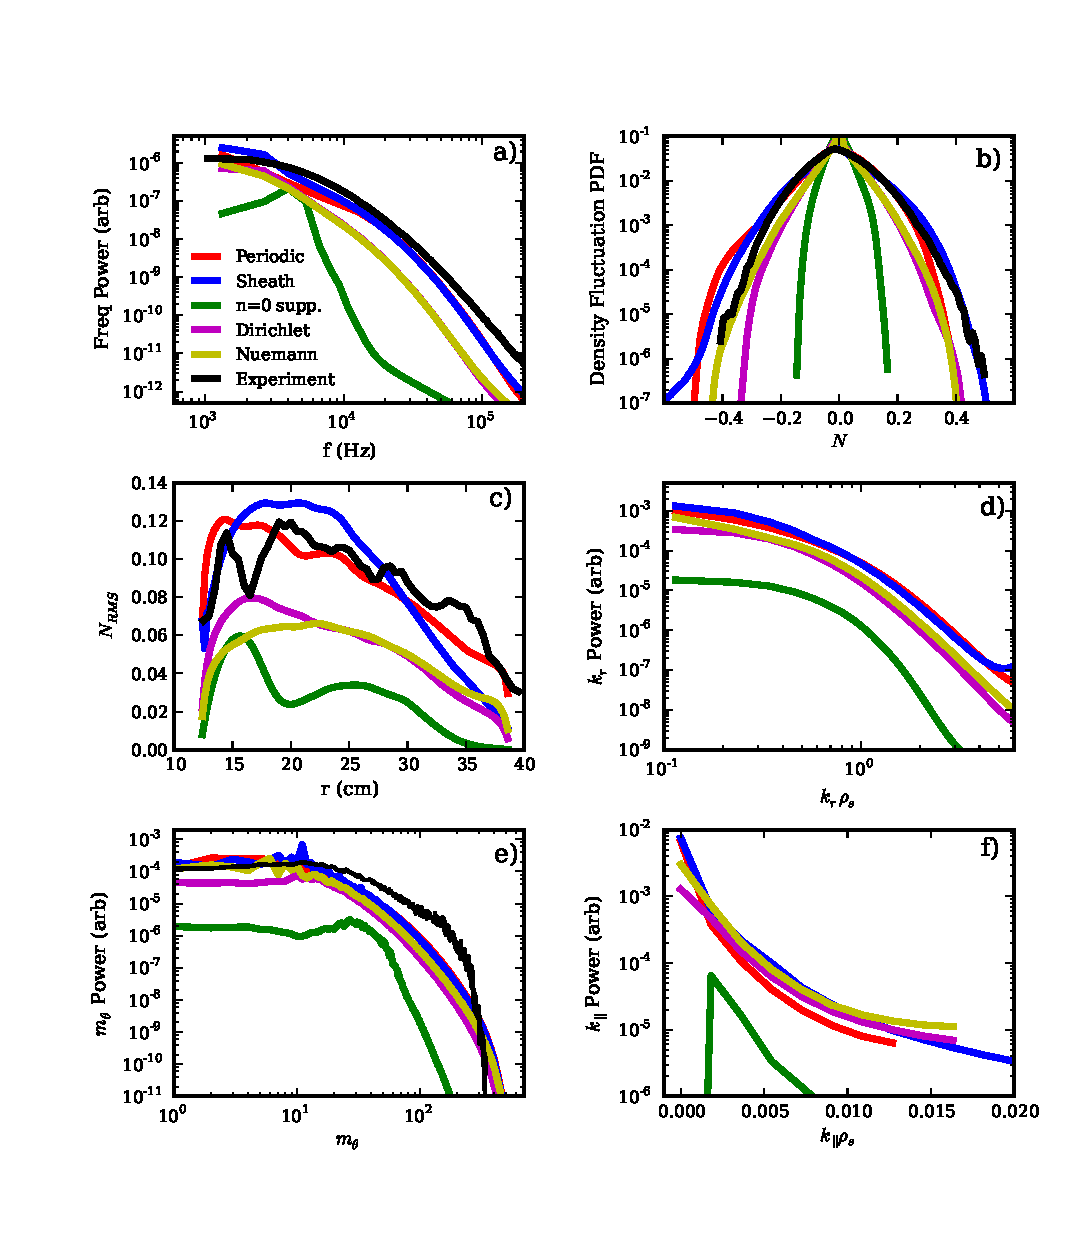
\includegraphics[]{n_statistics}}
\caption{Experimental and simulation fluctuation statistics}
\label{n_statistics_intro}
\end{figure}

In Chapter~\ref{c_lapd_turb}, I overview the results of the simulations. I begin showing linear instability growth rate curves, move onto the space-time evolution of the turbulence, and finally
show and discuss statistical properties of the turbulence. The analysis therein is simple, straight-forward, and model independent. I conclude from it that the simulations reproduce
statistical turbulent fluctuations that are statistically similar to those of the experiment in both a qualitative and quantitative manner, which validates the simulation model. 
Figure~\ref{n_statistics_intro} shows several statistical properties of the experimental and simulated turbulence that I also show in Chapter~\ref{c_lapd_turb}. 
The different curves -- other than that labeled ``Experiment'' -- correspond to simulations with different axial boundary conditions. 
It is clear that all but one of these simulations produces experimentally realistic turbulent fluctuation statistics. The one truly mysterious result, however, can be seen in
Fig.~\ref{n_statistics_intro} f). That is, all of the experimentally realistic simulations have axial wavenumber spectra that peak at $k_\para = 0$. The reason why this result is so interesting
is because the only linear instability in the simulations -- except for the Sheath simulation -- is the linear drift wave instability, which has positive growth rate only for finite $k_\para$.
The most unstable linear modes or waves generally dominate the structure of plasmas, but this isn't the case in these simulations.

To determine the origin of this unusual result, I analyze the simulations using energy dynamics.
Energy dynamics analysis use the simulation model as well as all of the spatial and temporal information output by the simulations to reveal dynamical processes such as 
energy injection into the fluctuations from the free energy equilibrium gradients, energy transfer between different waves or modes,
energy transfer between potential and kinetic energy degrees of freedom, and energy dissipation of the fluctuations. In Chapter~\ref{c_en_formalism}, I derive the energy dynamics equations for my
simulation model and explain which terms in the model correspond to the different processes. Specifically, I show that the terms involving advection of equilibrium variables
supply energy injection, the nonlinear advective terms cause mode to mode transfer, the adiabatic response terms transfer energy from potential to kinetic, and the collisional, diffusive,
and viscous terms supply the dissipation. Furthermore, I decompose the turbulent fluctuations in two bases: a partial Fourier basis and a Proper Orthogonal basis, and
I derive the energy dynamics equations for each of the basis functions.

\begin{figure}
\centerline{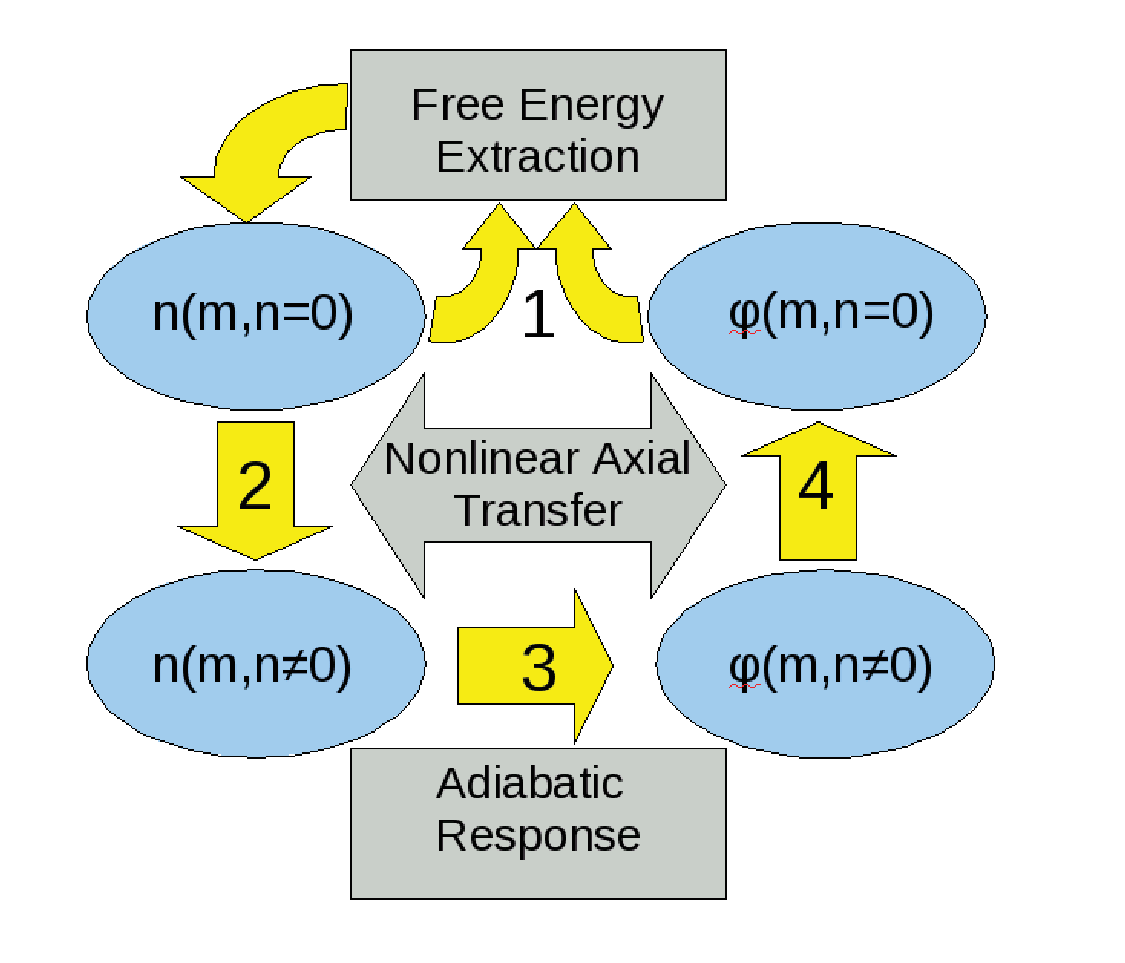
\includegraphics[]{reduced_nl_diagram}}
\caption{Nonlinear instability diagram}
\label{reduced_nl_diagram_intro}
\end{figure}

Then in Chapter~\ref{c_nlin_periodic}, by inputting the simulated turbulent results into the basis-decomposed energy dynamics equations, I uncover the primary mode-based processes that
control the turbulence including that which supports the $k_\para = 0$ fluctuations. In fact, the nonlinear instability 
cycle that supports the $k_\para = 0$ fluctuations is the most dominant process controlling the turbulence. I show a diagram of the cycle in Fig.~\ref{reduced_nl_diagram_intro}.
The process begins with the ``Energy Injection'' step, in which $k_\para = 0$ convective filaments or flute-like structures
advect density across the equilibrium density gradient, forming $k_\para = 0$ density fluctuations. 
These density fluctuations break up by axial three-wave transfer into finite $k_\para$ waves. An equivalent way to look at this step is that the azimuthal gradient that results from the density filaments
drives radially propagating drift waves that have finite $k_\para$. 
These finite $k_\para$ drift waves -- represented at the bottom of the diagram -- have access to the adiabatic response, 
meaning they can transfer energy between potential energy of the density fluctuations $N$ and the kinetic energy
of the potential $\phi$ fluctuations. The resultant drift waves then transfer some of their kinetic energy back to the convective filaments. 
This process is self-sustaining and it is necessarily nonlinear because it requires finite amplitude fluctuations to begin, and the three-wave transfers from the $k_\para = 0$ density fluctuations
to the drift waves and from the drift waves back to the convective cells are both purely nonlinear processes. 

Despite the nonlinear nature of the instability cycle, linear effects are still important because the nonlinearities of the system are energetically conservative.
This means that the energy that supports the process ultimately comes from a linear mechanism, specifically that in which the convective filaments advect density across the equilibrium density gradient. 
Such a process is unintuitive because all $k_\para = 0$ linear eigenmodes of the system are stable. This means that, individually, each $k_\para = 0$ eigenmode decays, losing energy to the equilibrium
gradient rather taking it.
Yet a linear process at $k_\para = 0$ still drives energy into the turbulent system. The process responsible for this is a transient growth mechanism unique to nonorthogonal
stable linear eigenmodes. Because the linear system is non-normal, the linear eigenmodes are not orthogonal to one another, and they are even be largely anti-parallel to each other.
When this happens, even when all of the eigenmodes decay, the system as a whole may still grow, although only transiently.  Nevertheless, this growth, when reinforced by nonlinear
effects, can sustain itself, continuing to drive energy into the system. I discuss this first in Chapter~\ref{c_turb_and_inst}, then again in
Chapter~\ref{c_nlin_periodic}. Interestingly, the nonlinear instability and the linear mechanism that drives it are analogous to those which drive turbulence
in many subcritical neutral fluid flows.

\begin{figure}
\centerline{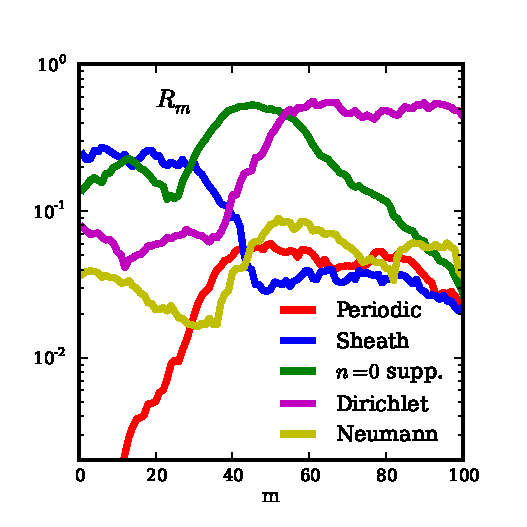
\includegraphics[]{lin_to_nl_ratios}}
\caption{Energy fraction contained in the most unstable eigenmodes}
\label{lin_to_nl_ratios_intro}
\end{figure}

While I focus only on the simulations that use periodic axial boundary conditions in Chapter~\ref{c_nlin_periodic}, in Chapter~\ref{c_nlin_nonper}, I generalize to the non-periodic simulations.
These merit a separate discussion because without the axial periodicity, the linear eigenmodes can have non-sinusoidal axial structures, or put another way, each eigenmode can have many non-zero
Fourier coefficients, including the Fourier coefficient of $k_\para = 0$. And, since the nonlinear instability is dependent upon $k_\para = 0$ effects, 
it can be more difficult to differentiate between linear and nonlinear instability in this case. I present arguments and analysis, however, supporting 
the robustness of the nonlinear instability in the simulations with non-periodic axial boundary conditions. One such analytical technique I use is determining the fraction of turbulent energy
contained in the most unstable linear eigenmode. I preview the result in Fig.~\ref{lin_to_nl_ratios_intro}, showing this fraction $R_m$ as a function of $m$ number. Except for a few places,
the fraction is less than $0.1$, indicating the small contribution of the linear instability in the turbulence.

\begin{figure}
\centerline{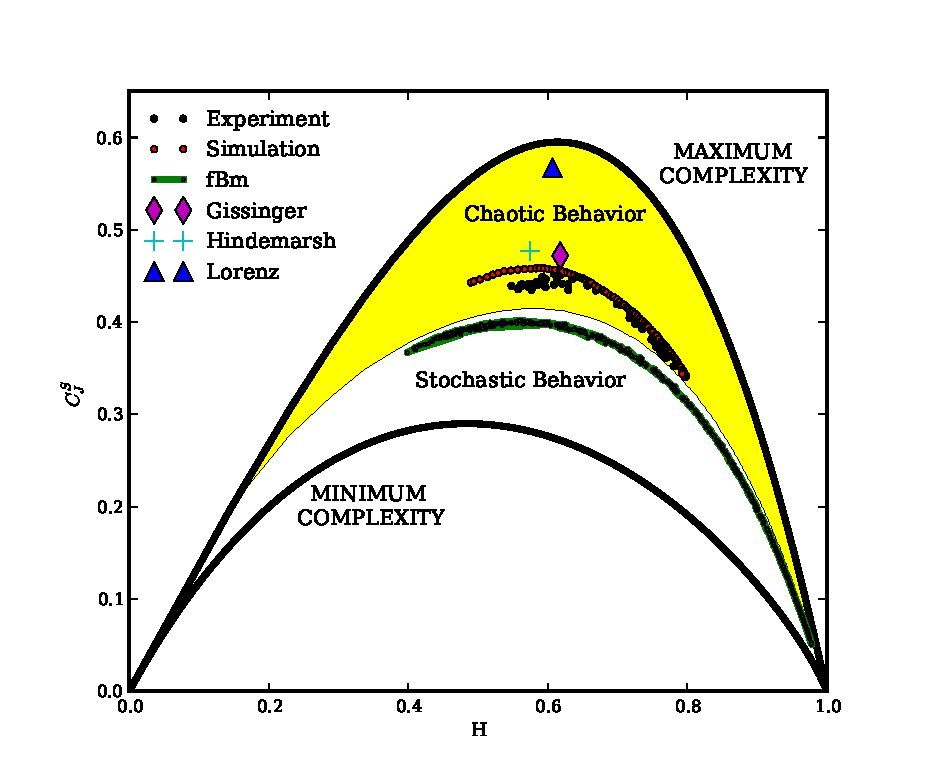
\includegraphics[]{entropy_complexity}}
\caption{Location of data in the entropy-complexity plane}
\label{entropy_complexity_intro}
\end{figure}

Finally, in Chapter~\ref{c_chaos}, I explore the deterministic, chaotic nature of the experimental and simulated turbulence. From Chapters~\ref{c_lapd_turb}-\ref{c_nlin_nonper}, I
use analytical techniques based on the statistical and structural nature of turbulence. These require a lot of information that can only be obtained from well-validated simulations.
But these don't answer deep questions regarding the solutions of the differential equations, like what is the dimensionality of the attractor solution? In fact, if the attractors are low
dimensional, meaning the turbulence is not stochastic, simpler analyses, highly reduced models, and non-simulation reconstruction techniques may be used to understand the turbulence.
So, in Chapter~\ref{c_chaos}, I attempt to find the dimensionality of the attractors. I do so first by exploring the temporal structure of time signals from experimental and simulation
observables. The Lorentzian pulse structure of the time signals indicates that the attractor may have low dimension, but more advanced analysis using permutation entropy techniques
reveals that this is not so. I show a result of the permutation entropy technique in Fig.~\ref{entropy_complexity_intro}, where I plot the permutation entropy against the permutation
complexity for experimental and simulation time signals along with other representative signals. The other time signals come from two low-dimensional chaotic models -- the Lorenz and Gissinger models --
and one stochastic model: fractional Brownian motion. Due to the relative location of the experiment and simulation in relation to the chaotic and stochastic models, it is evident that
the LAPD turbulence is stochastic, in this case meaning that it is high dimensional chaos. I further confirm this with a Proper Orthogonal Decomposition, which shows that many degrees of freedom are
active in the turbulence.
